%% Remaining TODO items:
%% - [X] make sure that code examples are finished (JMock needs work)
%% - [ ] adapt graphic descriptions of test patterns from xUnit book
%% - [ ] consider code examples of test pattersn besides mock objects
%% - [ ] consider changing the mock example to follow Freeman's turtle
%%       example

\chapter{Background}
\label{background}

In this section we will provide a brief tour of the OCaml programming
language, focusing especially on its powerful module system. The
chapter follows with a discussion of xUnit's Test Double patterns and
their implementation in OCaml and Java. The chapter concludes with a
summary of the current state-of-the-art testing tools for functional
languages such as OCaml and Haskell.

\section{A brief tour of OCaml and its module system}
\label{ocaml}

%% Define commands to change settings for Java and for OCaml. Need to
%% play with these more. Found this example at:
%% https://tex.stackexchange.com/questions/10141/how-to-prevent-lstlisting-from-splitting-code-between-pages
\lstnewenvironment{ocaml}[1][]%
  {\minipage{\linewidth} 
    \lstset{
      basicstyle=\ttfamily\footnotesize,
      language=ML,
      morekeywords={function,module,match,try},
      aboveskip=-\baselineskip,
      #1}}
  {\endminipage}

\lstnewenvironment{haskell}[1][]%
  {\minipage{\linewidth} 
    \lstset{
      basicstyle=\ttfamily\footnotesize,
      language=Haskell,
      morekeywords={function,module,match,try},
      aboveskip=-\baselineskip,
      #1}}
  {\endminipage}

\lstnewenvironment{java}[1][]%
  {\minipage{\linewidth} 
    \lstset{
      basicstyle=\ttfamily\footnotesize,
      language=Java,
      aboveskip=-\baselineskip,
      #1}}
  {\endminipage}

%% https://tex.stackexchange.com/questions/106844/adding-words-to-lstlisting-for-python-langaue
%% in order to get multiple levels of keywords
\lstset{
  language=ML,
  morekeywords={function,module,match,try},
  % Fix top/bottom frame margin spacing:
  % https://tex.stackexchange.com/questions/31598/lstlisting-produces-empty-row-when-used-inside-a-tabular
  aboveskip=-\baselineskip,
  %% framextopmargin=0pt,
  %% framexbottommargin=10pt,
  %% belowskip=10pt,
}

%% Want to talk quickly about code (functions, types, type inference),
%% modules, functors, first class modules. Mention that OCaml has a class
%% language, but that idiomatic OCaml typically uses functions and
%% modules unless a particular algorithm or solution to a problem
%% warrants an object-oriented implemtation.

OCaml is a strongly, statically typed functional programming language
based on the ML family of languages. It may be interpreted in a
read-eval-print loop called the OCaml ``toplevel,'' or it may be
compiled to an OCaml specific bytecode language or to a native
executable. \cite{ocaml:spec} It has a very good generational garbage
collector tuned for sequential programs. \cite{ocaml:gc_tutorial}

What follows is a \textit{very} brief tour of the OCaml programming
language. This should hopefully be enough to allow the reader to
follow along with the coding examples later in this chapter and the
next. For more assistance with OCaml, the reader is directed to the
OCaml Language Specification \cite{ocaml:spec}, and Real World OCaml
\cite{rwo}\footnote{Real World OCaml is available for free online:
  \url{https://realworldocaml.org}}

\subsection{OCaml basics: values, functions, and types}

\subsubsection{Values}

In OCaml, values are assigned to variables using the \code{let}
keyword.

\begin{lstlisting}
(* This is a comment *)
let num = 42
let str = "hello world"
let list = [1;2;3;4]
let tuple = (1,2)
\end{lstlisting}

Variables in OCaml are immutable, unless they are specially defined as
references, or mutable fields of a record type.

\begin{lstlisting}
let num = ref 42
Printf.printf "num was %d\n" !num
num := 24
Printf.printf "num is now %d\n" !num
\end{lstlisting}

\subsubsection{Functions}

Functions are created with the keywords \code{fun} or \code{function},
and assigned names using \code{let}, just like other values. Functions
defined using the \code{function} keyword can only take one argument,
but that argument can be pattern-matched.

\begin{lstlisting}
let f = fun a b -> a + b
let g = function
        | [] -> true
        | _  -> false
\end{lstlisting}

Functions can also be created using a shorthand \code{let} syntax. The
function \code{f} below is equivalent to the function \code{f} above.

\begin{lstlisting}
let f a b = a + b
\end{lstlisting}

Because functions are first-class values just like \code{int}s and
\code{string}s, we can pass them to other functions. For instance, the
function \code{List.map} takes a function \code{f} and a list
\code{ls}, and returns a new list containing the result of applying
\code{f} to each element of \code{ls}.

\begin{lstlisting}
let f x = x + 1
let ls = [1;2;3;4]
List.map f ls         (* returns the value [2;3;4;5] *)
\end{lstlisting}

\subsubsection{Types}

OCaml is a strongly, statically typed language. The compiler will
infer the type of values, and will return an error if a type
constraint is violated. For instance, the following function \code{f}
has type \code{int -> int -> int}, meaning that it takes two values of
type \code{int} and returns a value of type \code{int}. If a
\code{string} or \code{float} are passed to this function, a
compilation error is thrown.

\begin{lstlisting}
let f a b = a + b     (* has type int -> int -> int *)
f 40 2                (* this type-checks *)
f "4" "2"             (* this fails to type-check *)
f 41.8 0.2            (* this also fails to type-check *)
\end{lstlisting}

OCaml allows the user to define complex types.

\begin{lstlisting}
(* Tuples *)
type position = int * int

(* Variant types *)
type colours =
  | Red of int
  | Green of int
  | Blue of int

(* Record types *)
type book = {
  author : string;
  title  : string;
  mutable inventory : int;
}
\end{lstlisting}

%% type variables

Polymorphism in OCaml data types is expressed with type variables. In
the following example, \code{'a} is a type variable which can
represent any type, making \code{tree} a generic data type.

\begin{lstlisting}
type 'a tree =
  | Leaf of 'a
  | Node of 'a tree * 'a tree
\end{lstlisting}

\subsubsection{Polymorphic variants}

OCaml has a feature called \emph{polymorphic variants}. These are
similar to atoms or symbols in languages like Erlang or
Scheme. Polymorphic variants are distinguished from regular variants
by the backtick (\code{`}) preceding the label. Unlike regular
variants, polymorphic variants do not need to be capitalised, but this
is still common practice. A common use of polymorphic variants is to
encode inputs or outputs of functions; for instance, the below
function uses polymorphic variants for encoding success and failure
cases.

\begin{lstlisting}
let f = function
  | `String v ->
    Printf.printf "Got a string: %s\n" v;
     `Success
  | `Int v    ->
    Printf.printf "Got an int: %s\n" v;
    `Success
  | `Float _  ->
    print_endline "Wasn't expecting a float.";
    `Failure
\end{lstlisting}

Polymorphic variants can be used in the same way as regular variant
types, except that they don't need to be explicitly
declared. Furthermore, any polymorphic variant with the same name is
considered to be the same type (unlike regular variants, where
identically named constructors may be protected inside of different
modules, and therefore would be different types).

This gives rise to useful patterns in API development, such as
extensible API types. For instance, the Yojson library has an encoding
of standard JSON, as well as common, useful extensions to the JSON
spec. The standard JSON spec is encoded in \code{Yojson.Basic.json},
whereas the extensions to the standard are encoded in
\code{Yojson.Safe.json}. The \code{json} type in both modules uses
polymorphic variants to define the json grammar, and ``Basic'' JSON
can be easily upgraded to ``Safe'' JSON. A full treatment of this
library can be found in Chapter 15 of Real World OCaml \cite{rwo}.

\subsubsection{Pattern matching}

One of the most powerful features of languages like OCaml is pattern
matching. OCaml allows one to match over the structure of defined data
types. Pattern matching can be accomplished with the
\code{match value with | patt -> expr}
expression, or in functions created with the \code{function}
keyword. The following two functions are equivalent.

\begin{lstlisting}
let rec num_leaves_1 = function
  | Leaf _      -> 1
  | Node (l, r) ->
    (num_leaves l) + (num_leaves r)

let rec num_leaves_2 tr =
  match tr with
  | Leaf _      -> 1
  | Node (l, r) ->
    (num_leaves l) + (num_leaves r)
\end{lstlisting}

Note the use of the underscore (\code{_}) in the \code{Leaf}
pattern. In OCaml, underscore means ``match anything.'' It can also be
used in variable assignment, and is often used in module
initialisation code.

\subsubsection{Exceptions}

OCaml has exceptions that follow the usual ``try/catch''
pattern. OCaml exceptions have no ``finally'' clause, but this can be
implemented in a library using first-class
functions.\footnote{cf. \code{protect} and \code{protectx} in Jane
  Street's Core library:
  \url{https://ocaml.janestreet.com/ocaml-core/111.03.00/doc/core/\#Exn}}
Exceptions are declared similarly to variant data types.

\begin{lstlisting}
exception Not_found
let rec find x = function
  | [] -> raise Not_found
  | (k,v)::ls -> if x = k
                 then v
                 else find x ls
\end{lstlisting}

As with variants, exceptions can also carry data:

\begin{lstlisting}
exception Failure of string
exception Error of [`Invalid_request of string | `Permissions]
raise (Error (`Invalid_request "foo"))
raise (Error `Permissions)
\end{lstlisting}

``try/catch'' blocks in OCaml are similar to those in other languages,
except OCaml pattern matches on the ``catch'' block using the
\code{with} keyword.

\begin{lstlisting}
try
  raise (Error (`Invalid_request "foo"))
with
  | Error `Permissions ->
    print_endline "Bad permissions"
  | Error (`Invalid_request req) ->
    Printf.printf "Invalid request: %s\n" req
\end{lstlisting}

\subsection{The OCaml module system}

\subsubsection{Modules, signatures, and compilation units}

A distinguishing feature of OCaml is its powerful module system. A
module in OCaml is the basic compilation unit. Each compiled file is
assigned its own module. For instance, the definitions inside a file
called \code{foo.ml} would be placed into a module \code{Foo}.

%% XXX not sure if we want these to come from separate files, or if we
%% want to put a border around them, or...
%% \lstinputlisting[
%%   caption=foo.ml,
%%   %frame=single,
%% ]{code/foo.ml}
\begin{lstlisting}
type t = int
let f a = a
\end{lstlisting}

From outside of this module, function \code{f} would be referenced as
\code{Foo.f}. Module \code{Foo} has the following type:

\begin{lstlisting}
type t = int
val f : 'a -> 'a
\end{lstlisting}

The types of modules can be restricted using \code{mli} files. When
an \code{mli} file exists with the same basename as an \code{ml} file,
the module type of the module created for that \code{ml} file is
restricted to that of the signature specified in the \code{mli}
file. For instance, if \code{foo.mli} is:

%\lstinputlisting[caption=foo.mli]{code/foo.mli}
\begin{lstlisting}
type t = int
val f : ’a -> ’a
\end{lstlisting}

then the resulting type of module \code{Foo} would be:

\begin{lstlisting}
type t
val f : t -> t
\end{lstlisting}

Notice that \code{type t} is now abstract (meaning that we can't know
its implementation outside of module \code{Foo}, and function \code{f}
is now restricted to have type \code{t -> t}, instead of the more
general \code{'a -> 'a}.

OCaml modules can also be defined independently of compilation
units.

\begin{lstlisting}
module Bar =
struct
  type t = int
  let g a = a + 1
  let h ls = List.map g ls
end
\end{lstlisting}

We can also create module type signatures, which can restrict the
resulting type of a module in the same way as an \code{mli} file.

\begin{lstlisting}
module type BAR =
sig
  type t
  val h : int list -> int list
end
\end{lstlisting}

We can limit the type of \code{module Bar} to the signature
\code{BAR} by restricting it:

\begin{lstlisting}
module Bar2 = (Bar : BAR)
\end{lstlisting}

We can also restrict the original definition of \code{module Bar}:

\begin{lstlisting}
module Bar1 : BAR =
struct
  type t = int
  let g a = a + 1
  let h ls = List.map g ls
end
\end{lstlisting}

Modules \code{Bar1} and \code{Bar2} are now restricted by the
signature \code{BAR}. The value \code{g} is now hidden, and
\code{type t} is now abstract.

\subsubsection{Functors}

In most languages, a module system is primarily meant to provide a
namespacing system or a way to refer to compilation units
(cf. Haskell's module system \cite{www:haskell:modules}, or Python's
module system \cite{www:python:modules}). OCaml, however, has a much
more powerful module system, including the ability to define
\textit{functors}.

A functor is a relation from modules to modules. A functor can take a
module as an argument, and use it to specialise another module. For
instance, here is an example adapted from the OCaml language
``Introduction to OCaml'' \cite{ocaml:spec} that creates a \code{Set}
functor.

\begin{lstlisting}
module type ORDERED_TYPE =
sig
  type t
  val compare: t -> t -> int
end

module Set =
  functor (Elt: ORDERED_TYPE) ->
    struct
      type element = Elt.t
      type set = element list
      let empty = []
      let add x s = ...
    end
\end{lstlisting}

\code{Set} is a functor that takes some module with same type
signature as \code{ORDERED_TYPE}, and returns a module which is
specialised with that element type. For instance, we may create a new
\code{StringSet} module using the \code{Set} functor and the
\code{String} module from the OCaml standard library.

\begin{lstlisting}
module StringSet = Set(String)

let set = StringSet.add "foo" StringSet.empty in
StringSet.mem "foo" set  (* => true *)
\end{lstlisting}

For brevity, OCaml supports and alternative syntax for functor
definition which is more concise. For instance, we could have defined
the \code{Set} functor as:
\code{module Set(Elt : ORDERED_TYPE) = struct ... end}.
This comes in handy when one is defining a functor which takes
multiple arguments:
\code{module F(A : X)(B : Y) = struct ... end} .

Functors are useful for creating generic data types, such as the
\code{Set} type we defined above. We will soon see that they can also
be useful for dependency injection.

\subsubsection{First-class modules}

OCaml 4.00 introduced the feature of \textit{first-class modules}. A
first-class module is analogous to a language having first-class
functions: a module in OCaml can be packaged into a value, passed to
functions, and returned from functions. First-class modules provide a
similar capability as functors do, but are much more
light-weight. Refactoring a module into a functor can be a significant
amount of work, but adding a module argument to a function is a much
simpler change.

\begin{lstlisting}
module type DATABASE = sig ... end

module Db = struct ... end

let f db =
  (* Turn a module value into a module *)
  let module Db = (val db : DATABASE) in
  ...

(* And convert a module into a value *)
let _ = f (module Db : DATABASE)
\end{lstlisting}

\subsection{The rest of OCaml}

%% Briefly mention OCaml's object system and class language, and point
%% the reader to books and web resources.

In addition to the module language described above, OCaml also has a
rich class language and object system. Object orientation is a useful
addition to OCaml, but most OCaml code in practice eschews the use of
objects and classes. This dissertation will ignore the object oriented
features of OCaml and instead focus on its functional core and module
system. Most of the literature regarding software testing assumes
an object oriented implementation language; this dissertations
contributions lie elsewhere.

This was a whirlwind tour of OCaml. It was meant to cover just enough
syntax to get the reader through the OCaml examples in the next
section, and to understand the implementation in the following
chapter. For more extensive coverage, please see the OCaml language
spec \cite{ocaml:spec}, and the excellent Real World OCaml book
\cite{rwo}.

\section{Test Double patterns in detail}
\label{testdoubles}

%% XXX consider citing Gibbons \cite{gibbons:patterns}

\begin{figure}
  \centering
  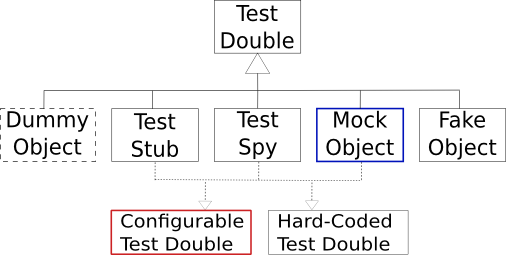
\includegraphics[scale=0.7]{img/test_double_taxonomy.png}
  \caption[Taxonomy of Test Double patterns]{Taxonomy of Test Double patterns\footnotemark}
  \label{fig:taxonomy}
\end{figure}
\footnotetext{Adapted from Meszaros \cite{meszaros:xunit}}

%%% (XXX) As figure \ref{fig:taxonomy} shows\dots

\begin{table}
  \centering
  \begin{tabular}{c|c|c|c|c|c}
    %% Header (in two parts for line-breaking)
    & Implements
    & Indirect
    & Indirect
    & Configurable
    & Behaviour
    \\
    & Interface
    & Inputs
    & Outputs
    &
    & Verification
    \\ \hline
    %% Rows
    \textit{Dummy} & No & No & No & No & No      \\ \hline
    Stub           & Yes & Yes & No & Yes & No   \\ \hline
    Fake           & Yes & No & No & N/A & No    \\ \hline
    Spy            & Yes & No & Yes & Yes & No   \\ \hline
    Mock           & Yes & Yes & Yes & Yes & Yes \\ \hline
  \end{tabular}
  \caption{Comparison of Test Double pattern features}
  \label{table:testdoubles}
\end{table}

Test Doubles allow developers to write tests that might have been
difficult or even impossible to write without a Test Double. As their
name suggests, Test Doubles are meant to stand in for a DOC of the
SUT. Their name is analogous to ``stunt doubles'' used in films to
stand in place for the main actor during dangerous scenes
\cite{meszaros:xunit}.

Meszaros describes three problematic scenarios for which Test Doubles
may be an appropriate solution.

\begin{description}

\item [Untested Requirement] A particular SUT may have a system
  requirement that needs to be exercised in a unit test, but testing
  this behaviour requires observing interactions between the SUT and
  one of its DOCs. If the DOC doesn't provide a mechanism for
  observing these inputs and outputs, a Test Double may be used in
  place of the DOC to observe the indirect inputs and outputs between
  the SUT and the DOC.

\item [Untested Code] A SUT may depend on a DOC which does not provide
  the test case enough control over its inputs to properly exercise
  the desired behaviour in the SUT. A Test Double for the DOC may be
  used in order to put the SUT into the state necessary to exercise
  this behaviour.

  Another instance of this issue occurs when the DOC has not been
  written yet, but a test for the SUT still needs to be written. This
  case often occurs in Test Driven Development (TDD) \cite{beck:tdd},
  where tests are usually written either before or during the
  development phase.

\item [Slow Test] Slow tests can be a major problem because they
  discourage the use of unit tests as part of the build process. A
  test may be slow because a particular DOC takes a long time to
  perform its task; perhaps it is performing a major calculation, or
  is downloading a file over a slow network connection. In this case,
  a Test Double may be used in place of the DOC in order to speed up
  the test cases which require this DOC.

\end{description}

\subsubsection{Indirect inputs and outputs}

Test Doubles have the benefit of being able to provide
\textit{indirect inputs} to the SUT, and to receive \textit{indirect
  outputs} from the SUT.

When exercising the SUT, we often need a way to control the
execution path of the SUT from the test case. In many cases, this is
not directly possible, because the SUT bases its execution path from
inputs received from one of its DOCs. These inputs are known as
\textit{indirect inputs}. In order to provide indirect inputs to the
SUT via the DOC, we can replace the DOC with a Test Double which
support indirect inputs (see table \ref{table:testdoubles}).

In order to verify that the SUT performed as expected during the test,
we may need to record the SUT's interactions with it's various
DOCs. These interactions are called \textit{indirect outputs} because
they are not directly visible from the test case itself. If a DOC does
not provide a way for the test case to read these indirect outputs in
a way that makes it possible to verify the correct behaviour of the
SUT, then a Test Double which supports indirect outputs may be used in
place of the DOC (see table \ref{table:testdoubles}).

\begin{figure}
  \centering
  
\includegraphics[scale=1.0]{img/indirect_inputs.png}
  \caption[Indirect Inputs]{Indirect inputs to a SUT\footnotemark}
  \label{fig:indirect_inputs}
\end{figure}
\footnotetext{Adapted from Meszaros \cite{meszaros:xunit}}

\begin{figure}
  \centering
  
\includegraphics[scale=1.0]{img/indirect_outputs.png}
  \caption[Indirect Outputs]{Indirect outputs from a SUT\footnotemark}
  \label{fig:indirect_outputs}
\end{figure}
\footnotetext{Adapted from Meszaros \cite{meszaros:xunit}}

\subsubsection{Common pitfalls of the Test Double patterns}

Using the Test Double patterns can make it easier to write unit tests,
but misuse of the patterns can cause problems. Because we are
replacing a DOC with a component that is custom-built for a particular
test case, we must be careful to avoid overly tight coupling between
the Test Double and the SUT. This can lead to \textit{Overspecified
  Tests}, which are a type of the \textit{Fragile Test} anti-pattern
\cite{meszaros:xunit}. A Fragile Test is one which may break due to
changes in the SUT which do not affect the behaviour being tested.

Another potential pitfall of misusing Test Doubles is the possibility
that the developer may accidentally replace the part of the SUT which
is being tested. This can be a severe problem, because tests for a
particular behaviour will show as passing, even though that behaviour
has never been exercised by the tests. Care should be taken when
writing tests to ensure that the test actually exercises the
behaviour under test.

\subsubsection{A note on terminology}

The xUnit Test Patterns book refers to the pattern as a \textit{Mock
  Object}. While OCaml does have object oriented features, we are
primarily concerned with mocking OCaml modules. In the rest of this
dissertation, we will use the term Mock Object when referring
specifically to the pattern described in the xUnit book, although we
mean to apply this pattern to OCaml's modules. When speaking of a
module that follows the Mock Object pattern, we may specifically refer
to this as a \textit{Mock Module}.

%% We will want to include diagrams relating all the test double
%% patterns, and describing them individually. The xunit web page has
%% many of these diagrams electronically, so we should use those where
%% we can, with proper attribution.

% http://xunitpatterns.com/Mocks,%20Fakes,%20Stubs%20and%20Dummies.html

%% XXX Should this go in a common definitions file? Probably...
\newcommand{\definition}[1]{\hangindent=1cm \textbf{#1}}

\subsection{Fake Object pattern}
\label{testdoubles:fake}

\definition{Fake Object} is a simpler version of the DOC which
performs the same function with less complexity.

A Fake Object is a simple replacement for a complex DOC. It does not
provide any test-specific features, such as the ability to deal with
indirect inputs or outputs. A Fake Object should be used when a SUT
has a complex DOC that makes it infeasible to run unit tests. For
instance, a web service DOC may be replaced by an object which returns
hard-coded results without the need to access the network. A database
may be replaced by a simpler data store such as a hash table or other
in-memory database.

%% TODO code example?

\subsection{Dummy Object pattern}
\label{testdoubles:dummy}

\definition{Dummy Object} is a special case of Test Stub which applies
to value types.

A \textit{Dummy Object} is a special case of a Stub Object. It is used
specifically when the SUT does not interact with the DOC at all during
the test, but a value for the DOC is still required in order to
initialise the SUT. For instance, the SUT may be a method of a class
which requires certain values to be constructed, but the SUT itself
doesn't make use of those values during the test. In a language with
nullable types, such as Java, a Dummy Object may simply be the
\code{null} value. In a language like OCaml, a Dummy Object may be a
value, such as a simple type constructor. A more complex type may have
a ``default'' or ``empty'' value that can be used. This is often the
case with record types, for which programmers often create an
``empty'' value which they can extend to create more complex
values. Many standard library containers have either an empty default
value, or a simple constructor, for instance \code{Set.empty} or the
value constructor \code{Buffer.create}, which takes a single integer
value.

%% A Dummy Object is used in place of a DOC when the SUT requires a
%% dependency for it's state, but the SUT doesn't use this dependency
%% during the test. It may be expensive to create a real instance of
%% the DOC, so a Dummy Object is created in its place. In languages
%% like Java, the \code{null} object may be used as a Dummy
%% Object. (What could we use in OCaml? Perhaps refactor so that the
%% DOC is an option type? OCaml types are often less complex than Java
%% objects, so we may have a simple constructor we can use instead of
%% null. A pattern we often use w.r.t. record types is to construct an
%% ``empty'' value of that type for later extension, so we could reuse
%% this value for testing purposes. Other than that, perhaps for
%% abstract types hidden within modules, we may have to provide a
%% ``dummy instantiator'' in that module (which is also a form of
%% refactoring for testability).)

%% TODO code example?

\subsection{Test Stub pattern}
\label{testdoubles:stub}

\definition{Test Stub} replaces a DOC in order to allow the test case
to provide \textit{indirect inputs} to the SUT.

The Test Stub pattern is the first of the Test Double patterns which
provides functionality specifically for the test case it is used
for. A Test Stub is an implementation of the DOC's interface which can
be programmed to provide indirect inputs to the SUT during the
test. This mechanism is used by the test case to provide indirect
inputs to the SUT via the DOC.

To use the Test Stub, the test case will configure a new Test Stub,
either at run-time by using stub generator from a testing framework,
or by creating a hard-coded Test Stub. The test stub is then inserted
into the SUT using some form of dependency injection. When the test is
run, the SUT receives indirect inputs from the test case via the Test
Stub DOC.

%% TODO code example?

\subsection{Test Spy Object pattern}
\label{testdoubles:spy}

\definition{Test Spy} replaces a DOC in order to record the SUT's
\textit{indirect outputs} and provide them to the test case.

The Test Spy is used to to replace the DOC in the SUT and record
the interactions that the SUT makes with the DOC. It is analogous to
the the Test Stub, but it works in the opposite way: instead of
providing indirect inputs from the test case to the SUT via the DOC,
it provides indirect outputs from the SUT to the test case via the
DOC.

The Test Spy is created in the same fashion as the Test Stub, and
inserted into the SUT in the same way. After the SUT has been
exercised, the test case may retrieve the SUT's indirect outputs from
the Test Spy and proceed with the evaluation of the test.

\subsection{Mock Object pattern}
\label{testdoubles:mocks}

\definition{Mock Object} combines the features of the Test Stub and
Test Spy to provide both \textit{indirect inputs} to the SUT and
record the SUT's \textit{indirect outputs}, as well as perform
\textit{behaviour verification}.

A Mock Object combines the features of a Test Stub and a Test Spy. It
is typically configurable at run time -- Mock Objects are usually not
hard-coded, at least in the languages for which there are Mock Object
frameworks. Mock Objects are capable of both providing indirect inputs
to the SUT, as well as recording indirect outputs from the SUT.

The single distinguishing feature of the Mock Object, which makes it
different than just a Test Double which behaves as both a Stub and a
Spy, is that it is capable of performing \textit{behaviour
  verification}. While a Test Spy simply performs the task of recording
the indirect outputs of the SUT for later reading by the test case, a
Mock Object provides facilities for verifying the correctness of the
indirect outputs from the SUT. A Mock Object may be either
\textit{strict} or \textit{lenient}. A strict Mock will raise a test
failure if it receives the wrong outputs (too few, too many, or an
unexpected output), as well as out-of-order outputs. A lenient Mock
may allow the test to pass if it receives at least the outputs it was
expecting, and may also allow out-of-order outputs. This behaviour
would be configurable by the the mocking framework.

%% XXX Consider just using the "turtle" example from Growing
\lstinputlisting[
    caption={Example of JMock, a Java Mocking framework},
    language=Java,
    label=code:jmock,
    aboveskip=\baselineskip,
  ] {code/java/jmock-example/src/test/java/JMockTest.java}

JMock is a mocking framework for the Java language. It is highly
configurable, and provides a domain specific language (DSL) for
configuring expectations \cite{freeman:evolving}. JMock's
expectation language provides many features beyond what is discussed
in the xUnit book. Listing \ref{code:jmock} is a small example of
using JMock, a Java mocking framework, in a test case.

\footnotesize
\begin{verbatim}
invocation-count(mock-object).method(argument-constraints);
  inSequence(sequence-name);
  when(state-machine.is(state-name);
  will(action);
  then(state-machine.is(new-state-name));
\end{verbatim}
\normalsize

Above is a pseudo-code notation of the expectation format that JMock
supports \cite{freeman:growing}. In addition to invocation counts and
method argument matchers and value returners, JMock provides both
\textit{sequences} and \textit{state machines} for use in mocks.

A sequence is a way of specifying that a series of invocations listed
in a mock's expectations are meant to occur in the specified order (a
\textit{strict} mock). Unless an invocation is added to a sequence,
the order of execution is not significant (a \textit{lenient}
mock). JMock also allows expectations to define simple state machines,
so that expectations can keep track of the state that the SUT should
be in during the test, and behave accordingly.

\section{Tools for software testing in functional langauges}
\label{testtools}

While much of the literature about and libraries for writing unit
tests are targeted at more-popular object oriented languages,
many functional languages also have testing libraries. Here is a short
summary of some of these libraries.

\subsection{xUnit implementations}

Unit testing frameworks for many languages follow the xUnit pattern of
testing (\cite{www:junit} \cite{www:nunit} \cite{www:ruby:unit}), and
languages like Haskell and OCaml are no different \cite{www:hunit}
\cite{www:ounit}. OCaml's OUnit is one of the more popular unit
testing frameworks for the language. It provides assertion functions
that can be used to verify that a test case has passed or failed,
combinators for grouping test cases into suites of tests, and helpers
for enabling or disabling individual test cases.

\lstinputlisting[
    caption=Example of OUnit usage,
    label=code:ounit,
    aboveskip=\baselineskip,
]{code/ounit_example.ml}

OUnit and HUnit both follow the xUnit Test Patterns guide for unit
tests, and therefor have the same feel as unit test libraries for
other languages, such as JUnit and NUnit, which are also based on the
xUnit patterns. The only major differences between these libraries is
that the OCaml and Haskell unit test libraries both use functional
combinators for building test cases and suites (the \code{>::} and
\code{>:::} operators in listing \ref{code:ounit}). Combinators such
as these are idiomatic to both of these languages.

Kaputt is another full-featured unit testing library for OCaml
\cite{www:kaputt}. In addition to supporting xUnit-style assertion
tests, it also supports QuickCheck-style specification testing.

\lstinputlisting[
    caption=Example of Kaputt usage,
    label=code:kaputt,
    aboveskip=\baselineskip,
]{code/kaputt_example.ml}

%% XXX Consider moving this paragraph to the QuickCheck section

As you can see from listing \ref{code:kaputt}, Kaputt's basic usage is
similar to that of OUnit, if not slightly more verbose. Kaputt also
supports specification-based testing, in the style of QuickCheck, as
shown in listing \ref{code:kaputt-spec}.

\lstinputlisting[
    caption=Example of Kaputt's specification-testing features,
    label=code:kaputt-spec,
    aboveskip=\baselineskip,
]{code/kaputt_specification.ml}

Kaputt also provides support for creating Mock functions, but this
part of the library is not as well developed as its assertion and
specification-based testing capabilities. Kaputt provides functions
for creating Mock functions which can record the number of times the
Mock has been called with a certain input value, and which can output
specified responses. It does not provide the ability to automatically
generate Mock Modules, nor does it provide capabilities for injecting
a Mock into a SUT. While it can record a SUT's indirect outputs, it
does not provide the ability to perform behaviour verification; this
must be performed manually by the test case. In this respect, Kaputt
provides features to aid developers in writing their own hard-coded
Mock functions, but little more.

\lstinputlisting[
  caption={Annotated example of Kaputt's mock
    features\protect\footnotemark},
  label=code:kaputt-mock,
  aboveskip=\baselineskip,
]{code/kaputt_mock.ml}

\footnotetext{Un-annotated example adapted from Kaputt's manual:
  \url{http://kaputt.x9c.fr/distrib/kaputt.html\#mock-example}}

In the example in listing \ref{code:kaputt-mock}, the call to
\code{List.map} is actually the SUT, and the function \code{succ} is
our DOC, for which we create the Mock \code{f}. This is a simplistic
example meant to demonstrate creating Mock functions using Kaputt, and
not to demonstrate proper testing procedure.

\subsection{Specification-based random testing with QuickCheck}

Koen Claessen's and John Hughes' ICFP paper ``QuickCheck: A
Lightweight Tool for Random Testing of Haskell Programs''
\cite{claessen:quickcheck} described a method of \textit{specification
  testing} that has since been ported to other languages, including
OCaml \cite{code:ocaml-quickcheck} \cite{www:kaputt}.

Specification testing is a method of describing the properties of the
SUT as specifications, and using random generators to attempt to
disprove the specification. For instance, say we want to test the
\code{reverse} function.\footnote{This is an example from Claessen's
  and Hughes' QuickCheck paper \cite{claessen:quickcheck}} This
function has the following properties:

\footnotesize
\begin{verbatim}
reverse [x]          = reverse [x]
reverse (xs++ys)     = reverse xs ++ reverse ys
reverse (reverse xs) = xs
\end{verbatim}
\normalsize

We can easily specify these properties in Haskell.

\begin{lstlisting}[language=Haskell]
rev_Unit x =
  reverse [x] == reverse [x]

rev_Append xs ys =
  reverse (xs ++ ys) == reverse xs ++ reverse ys

rev_Identity xs =
  reverse (reverse xs) == xs
\end{lstlisting}

And we can execute these specifications using quickCheck:

\footnotesize
\begin{verbatim}
Prelude Test.QuickCheck> quickCheck rev_Append

+++ OK, passed 100 tests.
\end{verbatim}
\normalsize

Specification testing is well suited to functional languages,
especially those which restrict or eliminate mutability and
side-effects, such as Haskell. It is common to write Haskell code
which separates side-effecting functions (those that operate under the
IO monad) from \textit{pure} functions which have no side
effects. These pure functions can then be tested using QuickCheck. 

\subsection{Criterion: Haskell benchmarking library}

While it isn't a unit testing library like HUnit or OUnit, Criterion
\cite{www:criterion} is a useful Haskell library for running
benchmarks. It is particularly interesting because of the attention to
statistical detail that the library provides. Each benchmark run is
calibrated against the system clock, and benchmarking runs with a high
degree of variance are flagged to the user.

\lstinputlisting[
    caption=Example of Criterion benchmark library,
    label=code:criterion,
    aboveskip=\baselineskip,
]{code/criterion_example.hs}

Below we see the command line output shown from running the code in
listing \ref{code:criterion}, while figure \ref{fig:criterion} is part
of the graphical output from running this program. In this image we
see that Criterion gives us both the raw time data (graph on the
right), and a kernel density estimate of the time data (graph on the
left).

\footnotesize
\begin{verbatim}
warming up
estimating clock resolution...
mean is 1.119713 us (640001 iterations)
found 65667 outliers among 639999 samples (10.3%)
  5404 (0.8%) low severe
  60263 (9.4%) high severe
estimating cost of a clock call...
mean is 58.35944 ns (7 iterations)

benchmarking fib/10
mean: 3.819773 us, lb 3.709738 us, ub 3.968785 us, ci 0.950
std dev: 653.0665 ns, lb 506.8601 ns, ub 834.0847 ns, ci 0.950
found 13 outliers among 100 samples (13.0%)
  6 (6.0%) high mild
  7 (7.0%) high severe
variance introduced by outliers: 92.538%
variance is severely inflated by outliers
\end{verbatim}
\normalsize

\begin{figure}
  \centering
  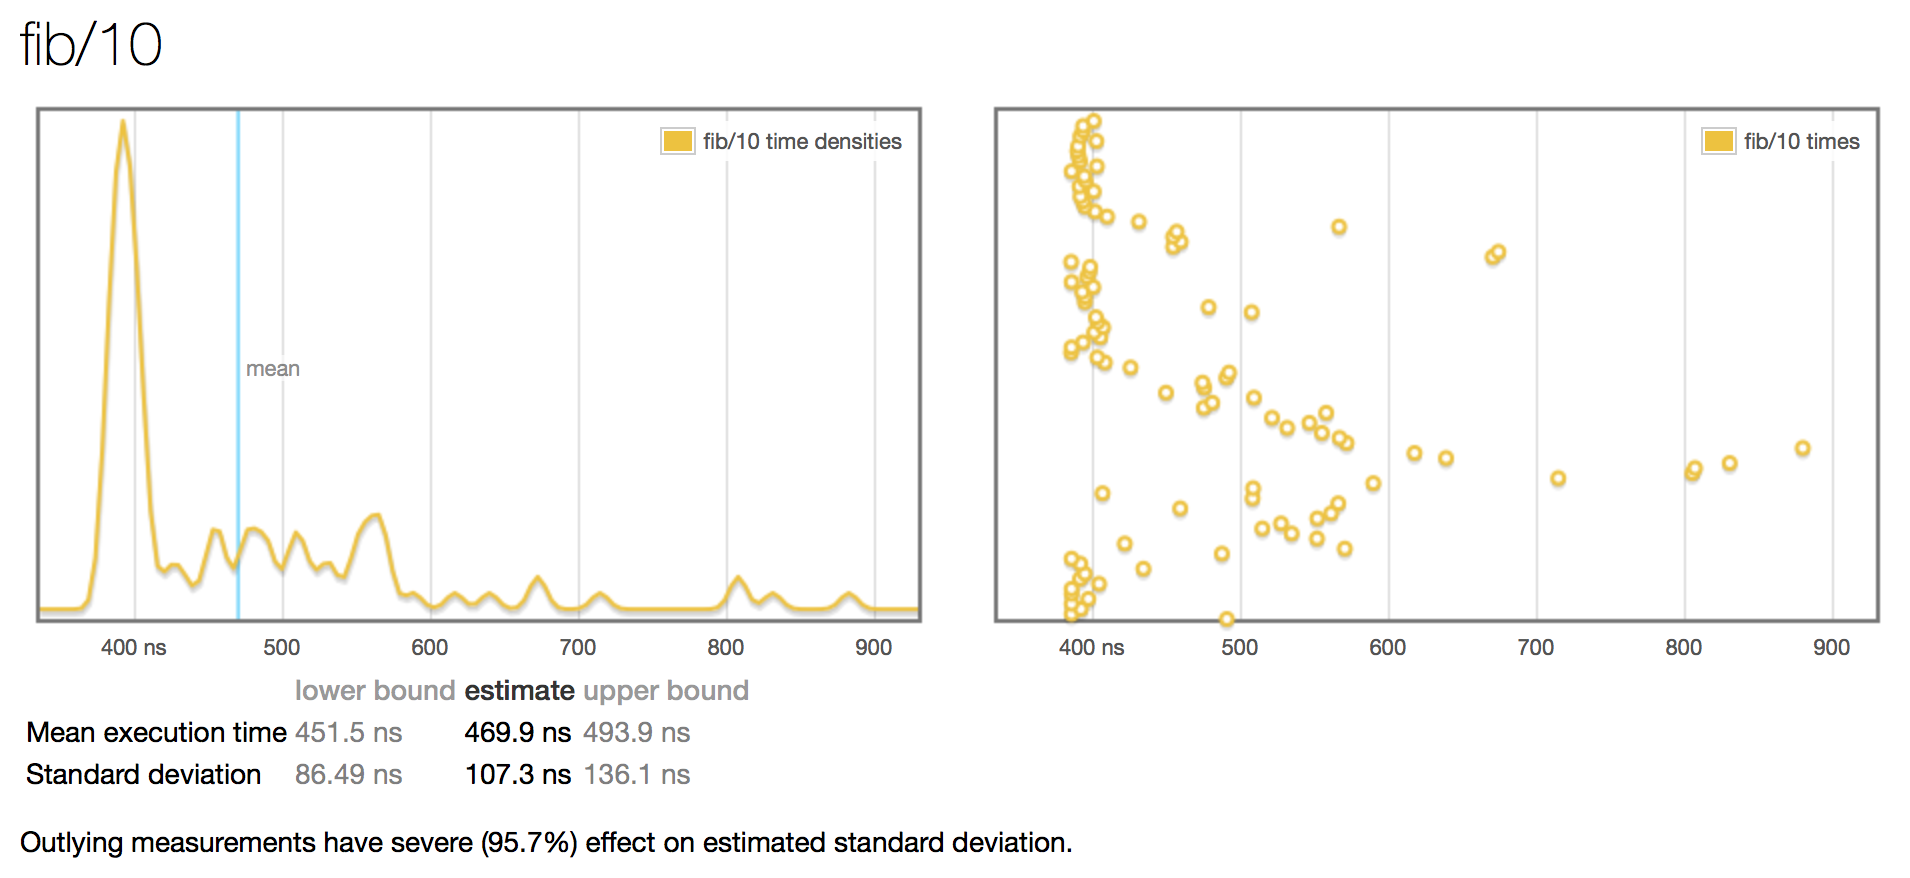
\includegraphics[scale=0.45]{img/criterion.png}
  \caption[Criterion Output]{Output from the benchmarking library Criterion}
  \label{fig:criterion}
\end{figure}

